% This file is based on the "sig-alternate.tex" V1.9 April 2009
% This file should be compiled with V2.4 of "sig-alternate.cls" April 2009

\documentclass{sig-alternate}

\usepackage{url}
\usepackage{color}
\usepackage{enumerate}
\usepackage{balance}
\permission{}
\CopyrightYear{2013}
%\crdata{0-00000-00-0/00/00}
\begin{document}

\title{CouchDB: A Comprehensive Review}
\numberofauthors{1}
\author{
\alignauthor
Anonymous
}
\date{}
\maketitle
\begin{abstract}
  With the rapid growth in the volume and variety of data, the need for effective systems for cheap and effective data management systems is on the rise. Data is collected from different sources. This data does not have tabular structure required by relational database system. This kind of semi-structured or unstructured data is usually has a short life-time. It is also necessary process this data quickly for generating actionable insights. It is not possible to allow the time required for designing a relational database system for this data. NoSQL database systems offer these advantages over the relational database system.

  This paper evaluates NoSQL based CouchDB database system. CouchDB is a document based database management system. This paper explores the technical details about CouchDB as well as its advantages over traditional database systems. We have discussed about the design philosophy of CouchDB which ensures effective data management system with built-in query engine with the advantage of being modular and scalable. Apart from that, we have also discussed about the data storage and query processing mechanism of CouchDB. CouchDB uses MapReduce concept for creating and maintaining views of stored data. In the latter part of the paper, view mechanism of CouchDB is explained. This paper attempts to provide, a comprehensive and detailed review of the CouchDB database management system.
\end{abstract}

\section{Overview}
\label{overview}
In this report, we will explore the details about the CouchDB system. In the recent years, the shear volume of generated data has increased significantly. While the volume of generated data is increasing rapidly, data storage has become cheaper. Organizations all over the world are storing as much data as they can. However, this data is collected at rapid rate. It has different structure. It not always possible to anticipated what would be the source of data in the near future. Data is collected from social networks, text messages, telephonic conversations and many other semi-structured or unstructured formats. It is very difficult to use the traditional data management techniques for managing this data. This rapid growth does not allow the time for understanding the structure of data, designing predefined schema and then processing the data. Most of this data has a short term usability. It is not feasible to invest large amount of resources for managing this kind of data.

In this report, we will discuss about the Apache CouchDB database system. CouchDB is a document based NoSQL database system developed by The Apache Software Foundation~\cite{couchDB}. In this report, we will present a comprehensive review about the CouchDB system from the point of view of design, data storage, retrieval and query processing.

\section{Relational Database vs NoSQL}
\label{relational nosql}
Section~\ref{overview} describes reasons which are driving forces behind the creation of NoSQL database systems. NoSQL database systems allows the storage and retrieval of data which is not present in tabular format. The traditional relational database systems always expect data to be modeled in tabular format. They are very powerful for managing that kind of data. However they required a lot of resources for designing the database and maintaining it. Relational databses usually require a databse administator for designing and maintaining the databse system. NoSQL databases stand for `Not only SQL'. They can have the query language support like the traditional relational database. However, they have the important characteristic of handling semi-structured or unstructured data without having to invest a large amount of time or financial resources.

With the continuous increase in generation of data, many NoSQL database management systems have emerged in recent past. NoSQL database systems use various approaches for designing the system. Most of the NoSQL database systems designed as column based, document based, key-value based or gram based system~\cite{wikiTypes}.

\section{CouchDB Characteristics}
\label{couchdb characteristics}
CouchDB is a document based NoSQL database~\cite{Anderson:CouchDB}. CouchDB handles the data which does not have tabular schema. CouchDB is designed to be a developer friendly database management system. Creators of CouchDB, Anderson et al.~\cite{Anderson:CouchDB} claim that the main features of CouchDB are schema free document model, built-in query engine, modularization and ease of scalability.

\subsection{Document Based Design}
\label{document based design}
In the real world, information is usually present as an integral structural unit. Consider a case of student transcripts. The transcripts have all the information about the student in one place. It has student name, id, courses taken, grades obtained and many other feature. People don't expect the real world information to be presented as different tables like relational database. The real world information is integrated and stored as a single unit.

CouchDB uses a similar approach for storage of data. All the data is stored in the form of documents in CouchDB. Each document represents a real world entity in the database. It is self contained and has complete information about that entity. It does not make any reference to some other document for the information about that entity like a relational database system. Any real world entity has to be represented within a single document. This makes the data storage process much simpler. Whenever you want to create new data, a new document is generated which is not dependent on any other document. Insertion and deletion of data is much easier with this document based approach of CouchDB.

Also real world entities have similar kind of information but they significantly differ with the information they represent. Anderson et al.~\cite{Anderson:CouchDB} have used an example of business card document in the real world. Business cards are created with the purpose of forwarding your contact information. They tend to have similar information about how to contact a person. However, means of contact differ significantly. Some business cards have fax number, cellphone number while other may not. If we want to model this information using traditional relational database system, we have to create the same field for each entry. In most of the cases that field will be blank. It is also possible that there might be many different fields of no significant importance. CouchDB does not have to deal with such kind of problem due to its document based structure. Since each document is integral structural unit independent of other documents. Each document can have fields which are only relevant to itself. It does not have to create extra blank fields like relational databases. Storing new data is significantly simplified because of this property.

\subsection{Built-in Query Processing Engine}
\label{query processing engine}
CouchDB has a built-in query processing engine. This engine uses Javascript for query processing. All the CouchDB documents are present in JSON format. CouchDB also returns the HTTP response in JSON format. It is possible to process simple JSON string using other programming language and use it for query processing.

CouchDB uses MapReduce concept for processing the queries. This concept uses a predefined map function and reduce function. These functions can be modified based on the structure of documents and query. This process allows the parallel index computation which provides a great flexibility. We will discuss the actual query processing in Section~\ref{query processing}.

\subsection{Modularization and Scalability}
\label{modularization and scalability}
Anderson et al.~\cite{Anderson:CouchDB} have claimed that CouchDB can handle different amount of traffic systematically. If CouchDB experiences large amount of traffic, it absorbs many concurrent requests. This assures that even though it make take a while,  all users will get there response without failing. This improves the reliability of CouchDB database systems.

CouchDB uses the MapReduce concept for evaluating results of a query. Map and reduce functions are applied to each document independent of each other. This ensures that the computation can be done parallaly and incrementally. CouchDB uses $B^{+}$-tree for storage of all the data as well as views. Since $B^{+}$-tree is sorted, it is ease to look for key-value pair even with a large amount of data.

The database access is managed using Multi-Version Concurrency Control (MVCC) in CouchDB. Any change that occurs in the document is appended at the end. Suppose there is a read request accessing a document. Concurrently a write request is issued for the same document. In relational databases, the resource is locked by the first read request. So the write request can't access the resource unless the read is complete. In CouchDB, the write request can access the document while it is being read by the first read request. The write request modifies the document and creates a new version of the document. This new version is appended at the end of the document. Any new read request coming after this point refers to this new version. However, the first read request is still valid because it is pointing towards the older version of the document. This removes the overhead required by the locking mechanism. In large database systems, sometime the locking mechanism takes more resources than the actual data processing requests. CouchDB scales effectively to such large databases due to MVCC framework. CouchDB is specifically designed for fault tolerance and better scalability. This makes the deployment of CouchDB for handling large amount of data easier.


\section{Data Storage}
\label{data storage}
CouchDB uses a data structure called $B^+$-tree for storing and indexing all of its data ans well as views. $B^+$-tree is used for storing large amount data. They provide quick access to data. The actual data is present at the leaf nodes of the $B^+$-tree. These leaf nodes are usually stored in the hard-drive. However, $B^+$-tree, usually, is not a deep tree. Due to this reason even though leaf nodes are present in hard-disk, upper level nodes are available in the main memory. $B^+$-tree is sorted tree. Using the upper level nodes which are present in the main memory, the actual data from leaf nodes can be extracted with few head seeks.

As explained in Section~\ref{modularization and scalability}, CouchDB uses MVCC for managing database access. Due to MVCC framework CouchDB avoid the overhead associated with locking mechanism. This has been implemented using append-only files. Older versions of file are not necessarily deleted when a newer version is created. Hence, all the requests always have a consistent pointer to the required data. Each document in CouchDB has an `\_rev' attribute. Based on the value of `\_rev' system ensures that only one request is changing one version.

CouchDB takes special care before committing any change to the file. Anderson et al.~\cite{Anderson:CouchDB} have explained that whenever any change occurs committing makes sure that database file is updated for reflecting changes. Committing is implemented using a footer which present in the last 4k of the file. The size of foot is 2k and it is written twice consecutively. Whenever any change occurs, CouchDB appends that change to file. It then check the length of the file and writes it in the first footer. CouchDB then pushes all the changes to the disk. Once all the changes are pushed, it copies the first footer into the second footer. Any failure can be checked using the difference between these footers. If any failure occurs the database can be restored to the consistent state by using non corrupt footer and pushing all the changes to the disk. This mechanism ensures the consistency of database at all the points.

\section{Query Processing}
\label{query processing}
CouchDB uses HTTP protocol for issuing queries to the CouchDB server. CouchDB provides 2 interfaces for processing query. CouchDB has a browser based interface called `Futon' which can be used for creating database, addition and deletion of documents and creating views. It also offers the curl utility for performing the same activities. We will discuss about the query processing in this section.

\subsection{Creating a Database}
\label{creating a database}
We have used the `curl' utility for creating the database. The format for this query is shown in Figure~\ref{fig:create}. This query is preformed using the verbose mode of curl. We will explain how the query works in the background using the logs printed on the screen. We have used PUT command for creating a new database. The `-vX' flag ensures that all the logs are printed on the console. The first 2 lines of logs, explain that curl is trying to establish a TCP connection and whether it is successful in creating that. We can be observed in Figure~\ref{fig:create} that first few lines of the logs start with asterisk. All these lines represent information about network connection and it success.

\begin{figure}
\centering
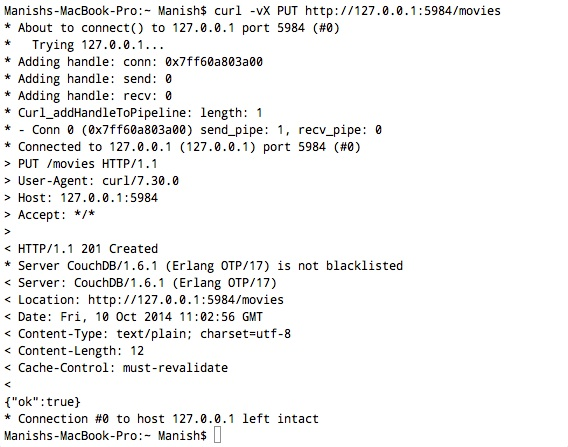
\includegraphics[width=90mm]{create.jpg}
\caption{Creating a Database \label{fig:create}}
\end{figure}

Next few lines of logs start with `>' or `<'. Character `>' represents that this command was sent to CouchDB by curl. On the other hand character `<' represents lines with were sent to curl by CouchDB. The first line with `>' marker calls the PUT method using HTTP request. Most of the information shown in Figure~\ref{fig:create} tell user what is going on behind the scene. All these processes are carried out by curl for which user doesn't have much control. Most of this information is useful for debugging some error in network connection or working of curl. However, the last line represents a JSON document. As we have discussed earlier, CouchDB stores all its data and views in JSON document format. It can be seen here that the result of any query made to CouchDB return the output in JSON format. In this case, it returns a simple document with one attribute. This result conveys a message to user that the database `movies' was successfully created. If there some error is encountered the final JSON response looks like \{"error":"not\_found","reason":"missing"\}. Based on this query response user can understand the reason behind failure of the query.

\subsection{Creating a Document}
\label{Create Document}
It has been mentioned in Section~\ref{document based design} that CouchDB uses documents as building blocks of system. All the documents are present in JSON format. In this section, we will discuss about query processing for creating the document in CouchDB. The query for document creation and its response is shown in Figure~\ref{fig:document}.

\begin{figure}
\centering
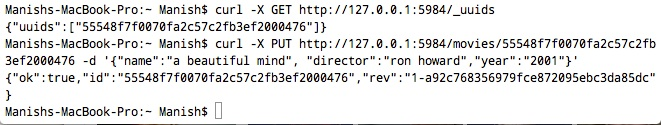
\includegraphics[width=80mm]{document.jpg}
\caption{Creating a Document \label{fig:document}}
\end{figure}

In Section~\ref{creating a database}, we have created `movies' database which is a collection of different movies. In this database, each movie is represented as an individual JSON document. Figure~\ref{fig:document} shows the query which creates one of such documents. Each document in the database has a unique key, which is known as id. This unique key is used as pointer for that document in database. User can create his own id. However, he has to make sure that each document is assigned a unique id. CouchDB solves this problem with `uuids' method. Using this method user can generate unique ids each time. The query for creating a new document calls PUT method. PUT method calls the URI of the movies database using an HTTP request. After this user has to provide the unique id for that document. The `-d' flag precedes the JSON document which contains all the required details.

This query return a JSON document which shows `id' and `rev' attributes. As discussed earlier, `id' represents the unique id. The `rev' attribute is used by CouchDB for MVCC based access control which has been discussed in Section~\ref{data storage}. Whenever the document is updated `rev' attribute is updated in order to represent updated version. The response ensures that the document has been created with the attribute ``ok'':``true''.

In Section~\ref{overview}, we have discussed the advantage of CouchDB over relational databases for handling the data which does not have tabular structure. The document shown in Figure~\ref{fig:document} contains fields like name, year and director. Some other movie may have attributes like plot, stars. These attributes can be incorporated in specific documents without affecting any other document. This is a good example of advantage offered by NoSQL database.

\subsection{Updating a Document}
\label{current status}
In this section, we will discuss about updating a document which is present in the database. While updating a document the most important attributes are `id' and `rev'. The `id' makes sure that curl has access to required document. curl uses the PUT method for updating the document in database. Figure~\ref{fig:update} shows the query for updating the document which is already present in the database.

\begin{figure}
  \centering
  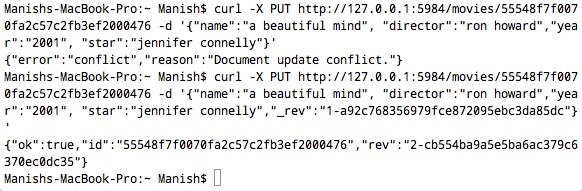
\includegraphics[width=80mm]{update.jpg}
  \caption{Update a Document
    \label{fig:update}}
  \end{figure}

We already have document for movie `A Beautiful Mind' in the movie database which has attributes like name, year and director. The query shown in Figure~\ref{fig:update} attempts to update this document with one more attribute named `star'. The first query tries to update the document directly by just adding the `star' attribute. However, CouchDB does not allow this query to modify the document. This happens because of the revision mechanism used by CouchDB. Revision mechanism is used for implementing the MVCC based access control and document storage. When a query wants to update a document, CouchDB needs that query to specify the current revision number of the document. Unless that number is specified, CouchDB does not allow the updation of the document. Once it has a pointer to the revision of the document, CouchDB access that revision and creates a new revision with the updated revision number. This mechanism ensures the consistency of the data throughout the system.

Documents in CouchDB can also have attachments of their own. These attachments can contain image file, other documents or anything like a real world document. Attachments get their own URL and they are just referenced when you query the document.

\section{Views}
\label{views}
CouchDB uses the concept of views for querying and reporting the CouchDB documents~\cite{couchDBviews}. Views are implemented using the MapReduce concept. CouchDB has 2 types of views. Permanent views are created by the user in the document called design document. These views are stored in the design document, in order avail frequently queried data rapidly. These views are created by the document designer. They depend on the characteristics of the data and application. Temporary views, on the other hand are created for on demand query execution. We have explained how the temporary views are created in CouchDB. We have used the same movie database with few more documents added to it.

CouchDB uses the Javascript language for creating views through MapReduce. We have written a map function which maps director to movies. Map functions emits the key, value pair of director and movie.\\
\begin{verbatim}
function(doc) { 
    if (doc.director && doc.name){
        emit(doc.director, doc.name);
  }
}
\end{verbatim}
The mapper checks whether a given document has director as well as name field. If both the field as present it emits a key-value pair (director, movie). This result is shown in Figure~\ref{fig:map}. Each pair has a name of the director as a key and name of the movie is value. Mapper function is applied to each document individually. We have combined the results yet obtained by mapper function. As we can see each key is associated with different values.
\begin{figure}
  \centering
  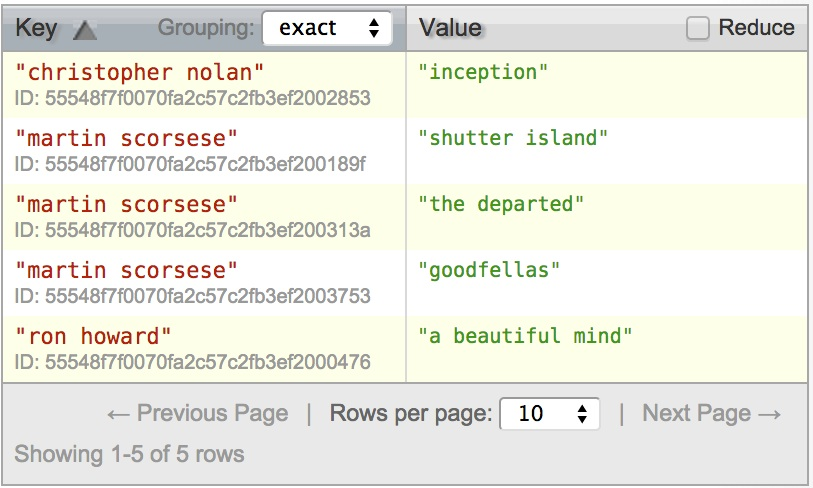
\includegraphics[width=80mm]{map.jpg}
  \caption{Map Function Output
    \label{fig:map}}
\end{figure}

Once we have result from mapper function, we can use a reducer function to combine all the results obtained from mapper.
\begin{verbatim}
function(key, values, rereduce) {
    return values;
}
\end{verbatim}
The reducer function appends all the movies by a single director to a single list. This gives us the final view where a key-value pair represents director as a key and list of all the movies directed by him as value. The result obtained by using reduce function are shown in Figure~\ref{fig:reduce}.
\begin{figure}
  \centering
  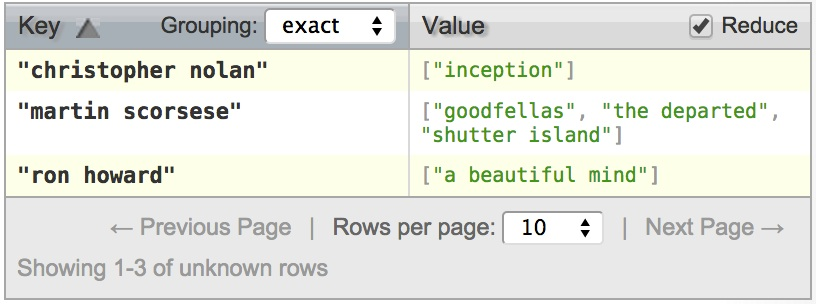
\includegraphics[width = 80mm]{reduce.jpg}
  \caption{Reduce Function Output
    \label{fig:reduce}}
\end{figure}
Both the views which are displayed here are temporary views which are calculated based on user query. Such views can be included in design document for faster performance. We have discussed about the design document in Section~\ref{design document}.

\section{Design Document}
\label{design document}
CouchDB stores all of its information in the form of JSON documents irrespective of whether it is data needed to be stored or views created by the user. CouchDB also stores the applications in the form document. These special kind of documents which are used for storing the application are called as design documents. These design documents contain JSON documents as well as views which are created by the designer. Anderson et al.~\cite{Anderson:CouchDB} have explained the basic structure of design document as follows,
\begin{verbatim}
{
  "_id" : "_design/movies
  "views" : {
      "map" : "function(doc){//do something}"
      "reduce" : "function(key, values, rereduce)
                                {//do something else}"
  }
}
\end{verbatim}
The design document has a unique id which identifies the document. This unique id starts with `\_design' to indicate that this is a design document. As shown in the code it has views created by map function and reduce function.

\section{Applications of CouchDB}
\label{applications}
This sections explains few applications which use CouchDB for their implementation. These applications use CouchDB because of several advantages offered by CouchDB.
\subsection{CouchDB for Update Notification}
\label{update notification}
It is one of the first Real time application developed using CouchDB. In relational database system, updating any database sends the notifications after it finishes the update process. These updates are affected by some changes made by the user. But in CouchDB,  there are two features that sends alert when there is some updates done by the user. First feature is to  send notifications by external process i.e. it reads an update notification by console and sends notifications. second feature supports sending notifications using "Changes" database-API.  This API checks if there is any change or update done at particular instance. One of the application of this feature can be observed in tweeting application. If a tweet needs to be posted urgently, then embed the document with ``urgent'' tag that notifies our twitter account as soon as it is added to CouchDB~\cite{twit}.

\subsection{Swinger}
\label{swinger}
Swinger~\cite{swinger} is a simple CouchDB application used to prepare and screen presentations online. This presentation slides can also be downloaded to system. The main application document is stored in CouchDB and query processing is done using javascript. Swinger  makes use of the CouchApp which is designed to support individual CouchDB applications that supports portability. CouchApp is a JQuery plugin that provides transparency for the CouchDB's document based approach.

\section{Summary}
\label{summary}
This paper provides a detailed review about CouchDB considering its various aspects. CouchDB has several advantages over relational databases when we have a large data-set with varying structure generated at a rapid rate. CouchDB has a robust model based on MVCC framework for access control and consistency. It also has a new approach based on MapReduce concept for indexing the data and creating output of queries. The paper explains the data storage, query format, consistency, query evaluation methodology of CouchDB. This paper helps readers in understanding the advantages and working of CouchDB.



\bibliographystyle{abbrv}
\bibliography{report}
% You must have a proper ".bib" file
%  and remember to run:
% latex bibtex latex latex
% to resolve all references
\balance
\end{document}








